\documentclass[a4paper, 11pt,abstract=on]{scrreprt}
\usepackage[utf8]{inputenc}
\usepackage[T1]{fontenc}
\usepackage[top=10pt, bottom=10pt, right=45pt, left=45pt]{geometry}
\usepackage{csquotes}
\usepackage[english]{babel}
\usepackage{float}
\usepackage{csquotes}
\usepackage{ulem}
\usepackage{fancyhdr}
\usepackage{lastpage}
\usepackage{blindtext}
\usepackage{tikz}
\usepackage{graphicx}
\usepackage{tikzpagenodes}
\usepackage{tabularx}
\usepackage{hyperref}
\usepackage[backend=bibtex,style=ieee]{biblatex}
\usepackage{enumitem}
\usepackage[color=red!100!green!33]{todonotes}
\usepackage{pdfpages}
\usepackage{lipsum}
\usepackage{ragged2e}

\addbibresource{doc.bib}
\bibliography{doc}
\graphicspath{{./img/}}


\title{Title}
\author{Vorname Nachname}
\date{\today}


\begin{document}

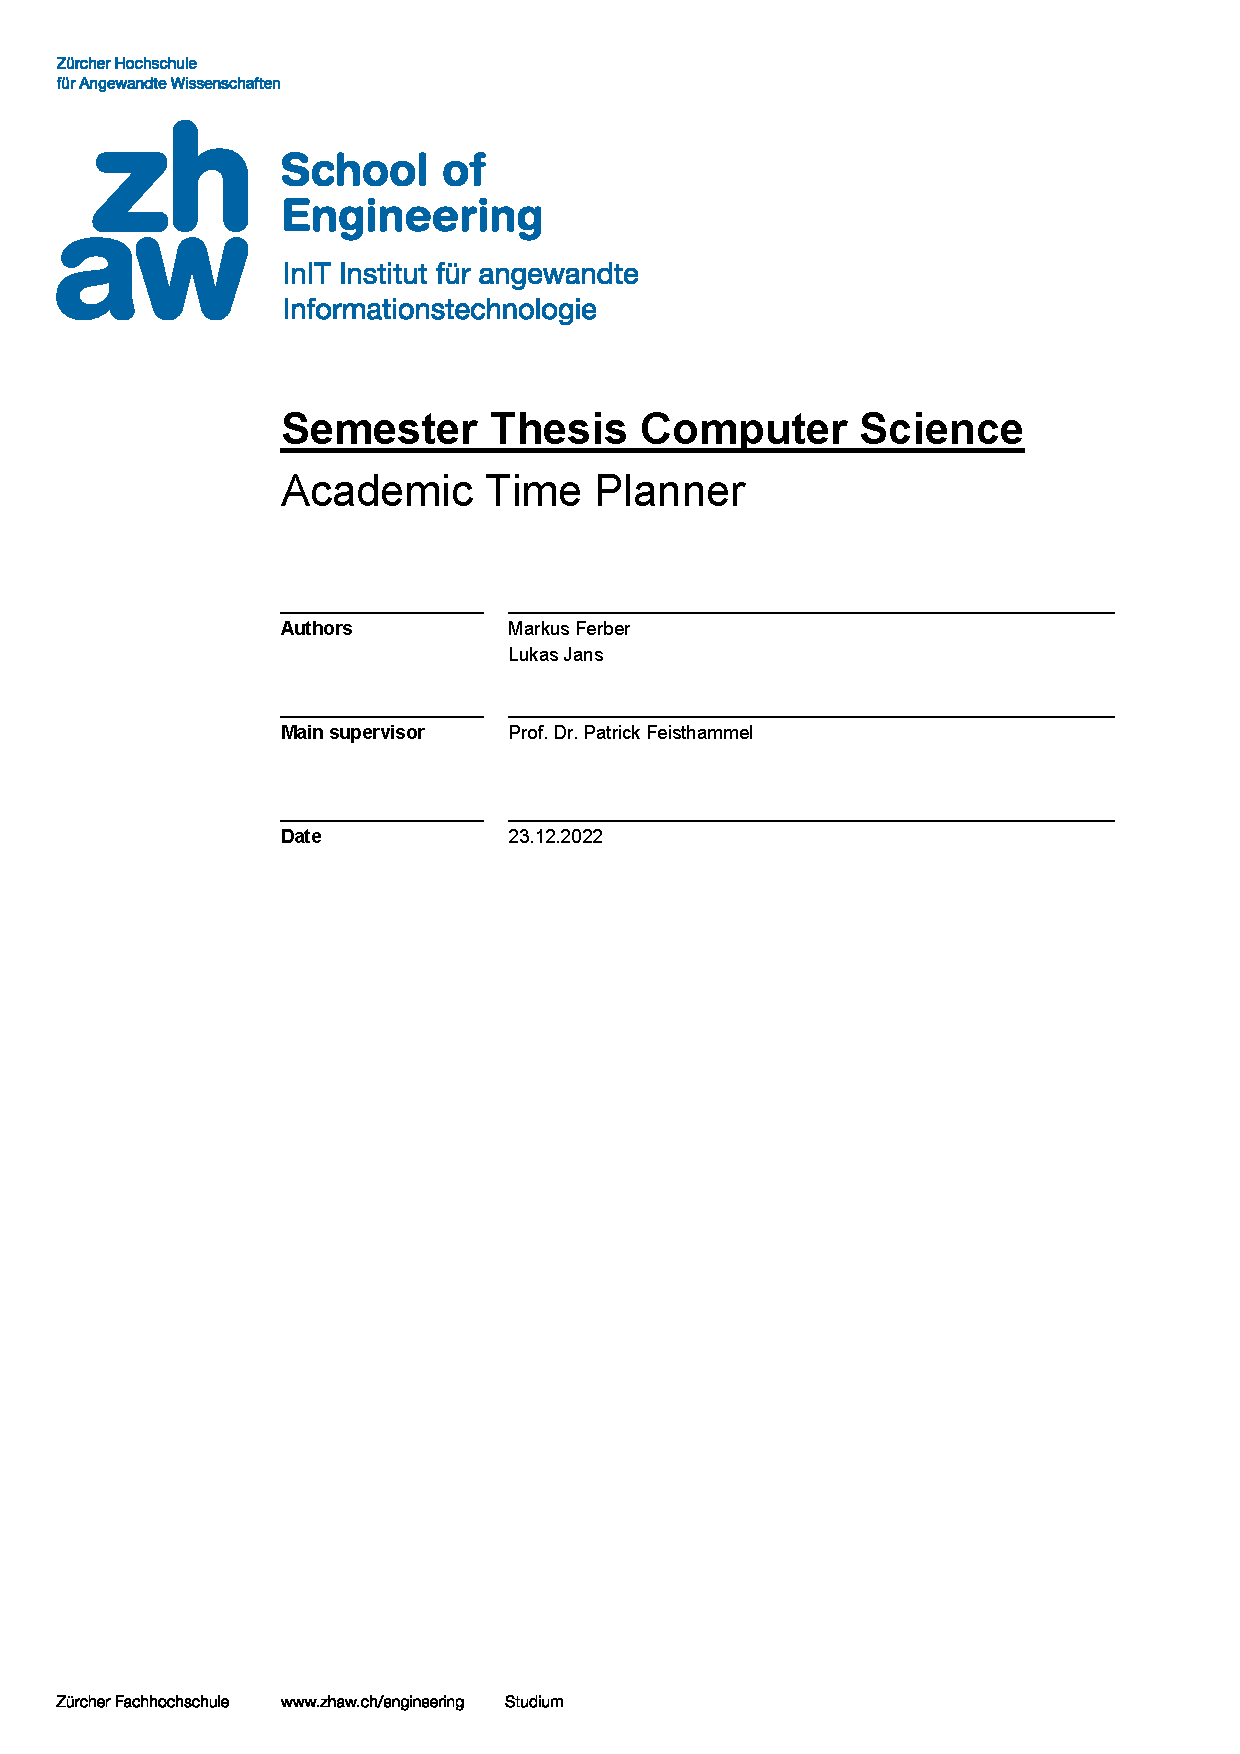
\includepdf{ressources/titlepage}

% Titelseite nicht als erste Seite zählen
\clearpage
\setcounter{page}{1}


\includepdf{ressources/Erklaerung_BA}

\selectlanguage{english} 
\begin{abstract}
%%% Local Variables:
%%% mode: latex
%%% TeX-master: "../doc"
%%% coding: utf-8
%%% End:
% !TEX TS-program = pdflatexmk
% !TEX encoding = UTF-8 Unicode
% !TEX root = ../doc.tex
\lipsum[1]

\end{abstract}

\chapter*{Preface}
%%% Local Variables:
%%% mode: latex
%%% TeX-master: "../doc"
%%% coding: utf-8
%%% End:
% !TEX TS-program = pdflatexmk
% !TEX encoding = UTF-8 Unicode
% !TEX root = ../doc.tex

This semester thesis was written by Markus Ferber and Lukas Jans in the fifth semester of their bachelor's degree in computer science at the Zurich University of Applied Sciences ZHAW in Winterthur. The authors would like to thank their supervisor, Patrick Feisthammel, as well as their additional advisor, Prof. Dr. Karl Rege, for their helpful advice and support throughout the realization of the thesis. They would also like to thank Mrs. Angelika Langham for her review of the thesis and her helpful remarks regarding the use of English language.\\
For the authors, this thesis presented a good opportunity to deepen their knowledge in software development. Many lessons could be learnt, in particular regarding the use of .NET technology and frameworks as well as the Fluxor design pattern.
\thispagestyle{empty}

\tableofcontents
\thispagestyle{empty}


\chapter{Introduction}
\setcounter{page}{1}
%%% Local Variables:
%%% mode: latex
%%% TeX-master: "../doc"
%%% coding: utf-8
%%% End:
% !TEX TS-program = pdflatexmk
% !TEX encoding = UTF-8 Unicode
% !TEX root = ../doc.tex

This section consists of the state of the art and the definition of the project. In the state of the art, the existing software prototype for this project and the approaches used for it are briefly explained. In the definition of project, the tasks and aims of the project are described, based on the definition provided by the supervisor.

\section{State of the art} \label{Initial position}
Toggl Track \cite{toggl_track_url} is an online application frequently used for time planning and tracking for projects or tasks. However, it does not provide the flexibility demanded by teachers and students in order to properly plan, track and compare their time efforts \cite{bachelorarbeit_Egger_Verstappen_page2}.
In the bachelor thesis on which this project is based, a technological prototype of an academic time planning software (Academic Time Planner, ATP) designed for complementary use with Toggl Track has been developed. The prototype has been realized as a .NET Blazor application fetching time data collected on Toggl Track via the Toggl Track Application Programming Interface (API). Moreover, a concept for mapping Toggl Track time data to ATP-specific time data as well as mockups for the graphical user interface (GUI) of the ATP have been evaluated.

\section{Definition of project}
Students and teachers have to organise their time for different tasks. The ATP is intended to support them in this matter, allowing for a semester-oriented time planning and helping to keep to the timing plans. To achieve this, the difference between planed time and used time should always be visible.
The time tracked is read via an API from the freely available time tracking application Toggl Track.
The goal of this project is to create a usable prototype based on the technological prototype already created and to realize the mapping concept, focussing on good and simple usability.
The prototype should be able to run locally and display an overview over the current difference between planed time and used time. Furthermore, it should include the state of the application as to whether the data fetched from Toggl Track is up-to-date and if there are any inconsistencies between ATP projects and Toggle Track projects. In addition to that, the import and export of planning data as well as the creation of plan projects via the application GUI should be made possible.
 




\chapter{Fundamentals}
%%% Local Variables:
%%% mode: latex
%%% TeX-master: "../doc"
%%% coding: utf-8
%%% End:
% !TEX TS-program = pdflatexmk
% !TEX encoding = UTF-8 Unicode
% !TEX root = ../doc.tex
\section{GitHub} \label{GitHub}
GitHub \cite{github_url} is an internet site which provides a Git based version control for software projects.
\subsection{Version control}
Version control is used to see what was changed when and by whom. It can also be used to roll back to an older state if needed. In GitHub a feature branch is used to implement the feature and then such a branch will be integrated into the main branch via a pull request. This pull request allows the other members of the team to request changes before the branch gets merged into the main branch. This process also allows members of a team to work independently without the problem of accidentally intervening with an other team members work.

\chapter{Methods}
%%% Local Variables:
%%% mode: latex
%%% TeX-master: "../doc"
%%% coding: utf-8
%%% End:
% !TEX TS-program = pdflatexmk
% !TEX encoding = UTF-8 Unicode
% !TEX root = ../doc.tex
\section{Organization Methodology}
For this project a reduced and modified version of SCRUM \cite{scrum_url} was chosen. These modifications include reducing the daily SCRUM meetings to two to three meetings a week, as we do not work on the project full time. One of these meetings was also attended by our project advisor Mr. Feisthammel. This meeting was usually held on Tuesday morning. There, a short progress report as well as the next weekly goals were discussed. Milestones as described in chapter \ref{Milestones} have been defined. They roughly correspond with the two-week sprint plan. An additional reduction is the absence of a sprint review as we do something similar in the weekly meetings described above. The point system as well as the burn down chart were also dropped.

\chapter{Results}
%%% Local Variables:
%%% mode: latex
%%% TeX-master: "../doc"
%%% coding: utf-8
%%% End:
% !TEX TS-program = pdflatexmk
% !TEX encoding = UTF-8 Unicode
% !TEX root = ../doc.tex
\lipsum[1]

\chapter{Discussion and prospects}
%%% Local Variables:
%%% mode: latex
%%% TeX-master: "../doc"
%%% coding: utf-8
%%% End:
% !TEX TS-program = pdflatexmk
% !TEX encoding = UTF-8 Unicode
% !TEX root = ../doc.tex
\lipsum[1]

\newpage

\addcontentsline{toc}{section}{Table of Figures}
\listoffigures

\addcontentsline{toc}{section}{Bibliography}
\printbibliography[title=Bibliography]
\end{document}